\section{Программная реализация}

После изучения алгоритма Тарского была начата работа по реализации этого алгоритма для формул без параметров.

\begin{definition}
    Формула $\mathcal{A}$ называется \textbf{формулой без параметров}, если для любой ее подформулы вида $(Qx)\mathcal{B}$, формула $\mathcal{B}$ свободна от вхождений кванторов и от переменных, возможно, за исключением переменной $x$.
\end{definition}

\subsection{Постановка задач}

Для поэтапного создания программы были сформулированы и решены следующие задачи:
\begin{itemize}
    \item Разработать архитектуру приложения, реализовать функции отдельных его блоков в виде интерфейсов;
    \item Реализовать систему, решающую задачу получения данных извне, например, из файла или консольного приложения;
    \item Реализовать систему, решающую задачу преобразования данных в формат, в котором формула будет выводиться экран или сохраняться в файл;
    \item Реализовать систему лексического и синтаксического анализов формул языка элементарной алгебры;
    \item Реализовать систему эквивалентных преобразований формул, реализовать алгоритм Тарского как одно из таких преобразований;
    \item Реализовать консольное приложение, которое применяет алгоритм Тарского к введенной формуле и выводит в консоль результат его работы;
    \item Покрыть основные модули программы модульными и интеграционными тестами.
\end{itemize}

\subsection{Инструменты разработки}

Для реализации алгоритма были выбраны язык C\# версии 9.0 и платформа .NET Core 5 \cite{TroelsonNet}. Такой выбор обусловлен рядом причин:
\begin{itemize}
    \item Язык C\#~--- это объектно-ориентированный язык программирования, а данная парадигма программирования позволяет абстрактно описывать объекты, в том числе и математические объекты; 
    \item .NET Core и .NET Standard~--- это современные, развивающиеся и востребованные кроссплатформенные технологии с открытым исходным кодом;
    \item Развитые и удобные средства параллельного программирования языка.
\end{itemize}

Написание программы осуществлялось в среде разработки Rider версии 2020.3. Доступ к программе был получен по студенческой лицензии (рис. \ref{fig:ide}).

\begin{figure}[ht]
    \begin{center}
        \begin{minipage}[ht]{0.8\linewidth}
            \center{\includegraphics[width=0.99\linewidth]{О IDE.PNG}}
        \end{minipage} 
    \end{center}
    \caption{Информация о среде разработки.}  
    \label{fig:ide}
\end{figure}

\subsection{Архитектура приложения}

В результате проделанной работы по проектированию приложения, исходя из предыдущего опыта создания программ, преобразующих логические формулы \cite{Gibadulin1}, было решено разделить программу на следующие слабосвязанные системы:

\begin{itemize}
    \item Система ввода~--- InputSubsystem. 
    
    Система выполняет функцию получения данных извне, например, из файла или консольного приложения;

    \item Система вывода~--- OutputSubsystem.

    Эта система решает задачу преобразования внутреннего формата представления формулы в человекочитаемый формат;

    \item Система парсинга~--- ParserSubsystem.
    
    Данный модуль методами лексического и синтаксического анализов из символьного представления формулы строит объект-формулу, с которой будут работать преобразователи. Также в этом модуле определяется реализация формулы как объекта; 

    \item Система эквивалентных преобразований~--- ProcessorsSubsystem.
    
    Данная система определяет реализации процессоров, то есть эквивалентных преобразований формул. В том числе здесь располагается реализация алгоритма Тарского;

    \item Консольное приложение для демонстрации результатов работы алгоритма Тарского.
    
    И наконец в этой части программы создано консольное приложение для демонстрации работы программы и алгоритма Тарского.

\end{itemize}
Взаимодействие между система происходит следующим образом:
\begin{itemize}
    \item Пользователь вводит с клавиатуры формулу в окне консольного приложения;
    \item Система ввода считывает эту формулу и передает в систему парсинга в виде последовательности символов;
    \item Система парсинга по последовательности символов строит объект средствами лексического или синтаксического анализов, представляющий собой формулу языка элементарной алгебры, и который умеют обрабатывать преобразователи;
    \item Система эквивалентных преобразований применяет процессоры, в том числе, алгоритм Тарского, для построения эквивалентной формулы. Полученная эквивалентная формула передаётся в системы вывода;
    \item Система вывода преобразует формулу в строковый вид, в котором она выводится в окно консольного приложения пользователю.
\end{itemize}

Далее рассмотрим каждую систему и её реализацию подробнее, при этом для наглядности будут приведены листинги исходного кода. В них будут отражаться члены классов или интерфейсов, а реализации конкретных методов будут пропускаться.

\subsection{Система ввода}

Система ввода должна решать получения данных извне, например, из файла или консольного приложения, и передачи эти данных в виде последовательности символов в систему парсинга.

\subsubsection{Интерфейсы}

Система ввода представлена интерфейсом IInput<T> (листинг \ref{IInput}). Интерфейс является обобщенным и ковариантным. Тип T должен реализовывать интерфейс ISymbol, который не содержит ни одного метода и ни одного свойства. Интерфейс содержит один метод MoveNext, который пытается перейти к следующему символу во входных данных и возвращает сигнал об успешности этого действия, то есть этот метод аналогичен одноименному методу интерфейса IEnumerator. Также интерфейс определяет два доступных только для чтения свойства: Current и IsOver. Первое возвращает текущий просматриваемый элемент входной последовательности. Второй истинно, если чтение входной последовательности завершено, иначе ложно.

Таким образом, интерфейс позволяет последовательно получать символы введенные пользователем в виде объектов типа T.

\lstinputlisting[label={IInput},caption={Интерфейс IInput<T>},captionpos=b]{../source/InputSubsystem/IInput.cs}

\subsubsection{Реализация}

Прежде чем перейти к реализации интерфейса IInput, предложим реализацию интерфейса ISymbol~--- класс Symbol (листинг \ref{Symbol}). Он предоставляет информацию о непосредственно символе и о его порядковом номере во входных данных.

\lstinputlisting[linerange={1-9,12-14},label={Symbol},caption={Класс Symbol},captionpos=b]{../source/InputSubsystem/Symbol.cs}

Интерфейс реализован классом TextReaderInput (листинг \ref{TextReaderInput}). Можно сказать, что класс является оберткой над классом System.IO.TextReaderInput. Во-первых, конструктор требует всего один аргумент типа TextReaderInput. В конструкторе инициализируются приватные поля класса и свойства интерфейса. Во-вторых, метод MoveNext при каждом вызове пытается прочитать очередной символ из \_textReader. Если прочитать символ не получилось или прочитанный символ является символом перевода конца строки, то чтение прекращается. Иначе в Current помещается новый объекта типа Symbol, полученный из прочитанного символа и текущего числа символов, счетчик символов \_symbolNumber увеличивается на один.

\lstinputlisting[linerange={4-12,17-20,31-37},label={TextReaderInput},caption={Класс TextReaderInput},captionpos=b]{../source/InputSubsystem/TextReaderInput.cs}

Непосредственно для ввода данных с консоли реализован класс ConsoleInput, который является классом наследником класса TextReaderInput (листинг \ref{ConsoleInput}).

\lstinputlisting[linerange={3-11},label={ConsoleInput},caption={Класс ConsoleInput},captionpos=b]{../source/InputSubsystem/ConsoleInput.cs}

А для чтения данных из файла~--- класс FileInput  (листинг \ref{FileInput}).

\lstinputlisting[linerange={3-16},label={FileInput},caption={Класс FileInput},captionpos=b]{../source/InputSubsystem/FileInput.cs}

\subsection{Система парсинга}


Система парсинга решает задачу лексического и синтаксического анализов формулы языка элементарной алгебры, а также определяет внутреннее представление формулы в виде объекта.


\subsubsection{Интерфейсы}

Объекты, определяющие внутреннее представление формулы языка элементарной алгебры, должны реализовывать интерфейс IExpression (листинг \ref{IExpression}). Единственный член этого интерфейса~--- readonly-свойство Type типа ExpressionType, которое определяет тип выражения: формула, терм или идентификатор, то есть литерал.

ExpressionType~--- перечисление (enum), которое имеет лишь три значения (листинг \ref{ExpressionType}). Эти значения несут информацию о том, какой тип имеет данное выражение языка: формула, терм или идентификатор соответственно.

\lstinputlisting[linerange={1-7},label={IExpression},caption={Интерфейс IExpression},captionpos=b]{../source/ParserSubsystem/IExpression.cs}

\lstinputlisting[linerange={1-9},label={ExpressionType},caption={Перечисление ExpressionType},captionpos=b]{../source/ParserSubsystem/ExpressionType.cs}

Следующая функция, которую выполняет система парсинга~--- построение внутреннего представления формулы по входной последовательности символов. Данная функция возложена на интерфейс IParser<TS, TE>~--- обобщенный ковариантный по первому, контравариантный по второму типу интерфейс (листинг \ref{IParser}). Первый тип должен реализовывать интерфейс ISymbol, второй~--- IExpression. Интерфейс определяет всего один метод Parse, который по входным данным типа IInput<TS>, на выходе отдает объект типа TE. Иначе говоря, эта функция преобразует введенную строку во внутреннее представление логических выражение.

\lstinputlisting[linerange={3-9},label={IParser},caption={Интерфейс IParser},captionpos=b]{../source/ParserSubsystem/IParser.cs}

\subsubsection{Реализация}

Интерфейс IExpression реализует класс SyntaxTree (листинг \ref{SyntaxTree}). Класс содержит readonly поле Token типа Token, три readonly свойства OperandsCount, Operands, Type, один метод и единственный конструктор. Из имени класса очевидно, что для внутреннего представления формул используется дерево синтаксического разбора. Пройдемся по членам этого класса.

В дереве синтаксического разбора каждая вершина отмечена терминальным символом, которые мы будем называть токенами. Класс Token~--- абстрактный класс, являющийся классом наследником класса Word, новых членов по сравнению с родительским классом не добавляет (листинг \ref{Token}). В свою очередь класс Word также является абстрактным, абстрактно переопределяет метод ToString (листинг \ref{Word}).

\lstinputlisting[linerange={5-16,19-22,28-32},label={SyntaxTree},caption={Класс SyntaxTree},captionpos=b]{../source/ParserSubsystem/SyntaxTree.cs}

\lstinputlisting[linerange={1-7},label={Token},caption={Класс Token},captionpos=b]{../source/ParserSubsystem/Token.cs}

\lstinputlisting[linerange={1-7},label={Word},caption={Класс Word},captionpos=b]{../source/ParserSubsystem/Word.cs}

Свойство OperandsCount, очевидно из названия, определяет количество операндов, то есть, количество дочерних вершин. Сами операнды расположены в неизменяемом массиве Operands, элементы которого также имеют тип SyntaxTree. Метод GetOperand возвращает операнд по его номеру.

В классе SyntaxTree определен единственный конструктор, принимающий на вход тип выражения, токен и массив операндов.

И последний член этого класса~--- Type, реализует соответствующее свойство интерфейса.

Переходим к классу SyntaxTreeParser, который реализует интерфейс IParser, а точнее IParser<Symbol, SyntaxTree> (листинг \ref{SyntaxTreeParser}).

\lstinputlisting[linerange={6-9,12-13,17-24,36-37,72-73,76-77,382-383},label={SyntaxTreeParser},caption={Класс SyntaxTreeParser},captionpos=b]{../source/ParserSubsystem/SyntaxTreeParser.cs}

Верхнеуровнево, метод Parse реализован следующим образом: по последовательности входных символом строится последовательность лексем методами лексического анализа, затем из последовательности лексем получается синтаксическое дерево методами синтаксического анализа. Теперь подробнее разберем как проводится разбиение на лексемы и каким образом строится синтаксическое дерево.

Прежде чем перейти к этапу лексического анализа, необходимо сказать о классе Lexeme (листинг \ref{Lexeme}). Этот класс является абстрактным, абстрактно переопределяет метод ToString родительского класса Word, а также содержит два readonly свойства FirstSymbolIndex и LastSymbolIndex, которые хранят информацию об индексе относительно входных данных первого и последнего символа, образующих лексему.

\lstinputlisting[linerange={1-10},label={Lexeme},caption={Класс Lexeme},captionpos=b]{../source/ParserSubsystem/Lexeme.cs}

Конкретными реализациями абстрактного класса Lexeme являются классы LiteralLexeme и SpecialSymbolLexeme. Первый определяет лексемы состоящие только лишь из букв и символов, то есть литералы. Эти последовательности также могут начинаться с символа обратного слэша. Второй~--- остальные символы, кроме обратного слэша. В то время как LiteralLexeme хранит информацию о литерале в виде строки, класс SpecialSymbolLexeme хранит информацию лишь об одном символе типа Symbol. 

Разбиение на лексемы производится достаточно стандартным образом:
\begin{itemize}
    \item пропускаются все пробельные символы, они лишь являются разделителями;
    \item последовательности из чисел и букв, возможно, начинающиеся с символа обратного слэша, образуют лексемы-литералы;
    \item остальные символы~--- лексемы-спецсимволы.
\end{itemize}

Напомним, что реализован синтаксический разбор в методе ToSyntaxTree. Если для языка элементарной алгебры построить контекстно-свободную грамматику, то методом рекурсивного нисходящего разбора\cite{Sokolov} можно построить дерево разбора. Реализовать этот метод нетрудно, нужно лишь научиться сопоставлять лексемы токенам, и для каждой группы правил с одинаковой левой частью написать функцию, которая последовательно пытается применить каждое из правил. Также эти функции, подобно машине Тьюринга, должны иметь возможность обозревать последовательность лексем, перемещаясь по этой последовательность вправо или влево. Каждая из этих функций в нашей реализации на вход принимает параметр типа ParsingContext, который позволяет просматривать последовательность лексем, разбивать ее на подпоследовательности, а также реализует подсчет баланса скобок. А возвращают эти функции одну из реализаций абстрактного класса Token: IdentifierToken или OperatorToken. Токены первого типа~--- это константы или переменные, а второго~--- остальные символы алфавита языка элементарной алгебры, а также два новых символа для нульместных предикатов (листинг \ref{OperatorToken}).

\lstinputlisting[linerange={11-26},label={OperatorToken},caption={Соответствие OperatorName и строкового представления},captionpos=b,literate={∃}{$\exists$}1 {∀}{$\forall$}1 {∨}{$\lor$}1 {→}{$\to$}1 {¬}{$\lnot$}1]{../source/ParserSubsystem/OperatorToken.cs}

При этом можно реализовать ряд эвристик, чтобы уменьшить временную сложность алгоритма нисходящего разбора вплоть до линейной или квадратичной. Например, можно использовать понятие баланса скобок, благодаря чему находить ведущий операнд. В нашей реализации была достигнута именно квадратичная от длины входной строки временная сложность, чего с запасом достаточно для нашей задачи. Действительно, алгоритм Тарского имеет сверх экспоненциальную временную сложность, поэтому быстрая обработка длинных строк неактуальна в нашем случае, хотя и возможна.

И наконец, выпишем  в форме Бэкуса--Наура\cite{Sokolov} грамматику языка элементарной алгебры. В этой грамматике учтено, что возведение в степень обладает правой ассоциативностью, в то время как остальные бинарные операции лево-ассоциативны. Также в эту грамматику заложен приоритет арифметических операций.

\begin{grammar}

    <формула> ::= <кванторная ф-а>  

    <кванторная ф-а> ::= (<квантор><переменная>)<кванторная ф-а>
    \alt <ф-а с бин. связкой> 

    <ф-а с бин. связкой> ::= <ф-а с бин. связкой><бин. связка><ф-а с ун. связкой>
    \alt <ф-а с ун. связкой>
    
    <ф-а с ун. связкой> ::= <унарная связка><ф-а с ун. связкой>
    \alt <предикатная ф-а>

    <предикатная ф-а> ::= <терм><предикат><терм>
    \alt (<формула>)

    <квантор> ::= \textbackslash exists
    \alt \textbackslash forall

    <бин. связка> ::= \textbackslash land
    \alt \textbackslash lor
    \alt \textbackslash to

    <унарная связка> ::= \textbackslash not

    <предикат> ::= \textgreater
    \alt \textless
    \alt =

    <терм> ::= <+- терм>

    <+- терм> ::= <+- терм><плюс минус><*/ терм>
    \alt <*/ терм>

    <плюс минус> ::= +
    \alt -

    <*/ терм> ::= <*/ терм><умножение деление><exp терм>
    \alt <exp терм>

    <умножение деление> ::= *
    \alt /
    \alt \textbackslash over

    <exp терм> ::= <- терм><возв. в степень><exp терм>
    \alt <- терм>

    <возв. в степень> ::= \string^

    <- терм> ::= <минус><- терм>
    \alt <литерал>

    <минус> ::= -

    <литерал> ::= <переменная>
    \alt <нат. число>
    \alt (<терм>)

    <переменная> ::= <буква>
    \alt <буква>\_<нат. число>

    <буква> ::= а | б | ... | я 
    \alt А | Б | ... | Я
    \alt a | b | ... | z
    \alt A | B | ... | Z

    <нат. число> ::= <цифра>
    \alt <цифра><нат. число>

    <цифра> ::= 0 | 1 | ... | 9
    
\end{grammar}

Если в ходе разбора не удалось применить ни одно из правил, то бросается исключение с информацией об возможной ошибке, допущенной при вводе формулы.

\subsection{Система вывода}

Система вывода решает задачу преобразования данных в формат, в котором формула будет выводиться экран или сохраняться в файл.


\subsubsection{Интерфейс}

Возложенная на систему вывода функцию описывает обобщенный контравариантный интерфейс IOutput<TE>, где тип TE должен реализовывать интерфейс IExpression (листинг \ref{IOutput}). Интерфейс содержит единственный метод Print, который по выражению строит его строковое представление.

\lstinputlisting[linerange={3-9},label={IOutput},caption={Интерфейс IOutput},captionpos=b]{../source/OutputSubsystem/IOutput.cs}

\subsubsection{Реализация}

Интерфейс IOutput<SyntaxTree> реализован классом NativeOutput. Не будем вдаваться в подробности реализации этого класса. Но отметим, что он преобразует формулу в строку учитывая приоритет операций, их арность, нотацию записи и левую или правую ассоциативность. 

Для вывода кванторов, пропозициональных связок и других особых символов используются соответствующее символы юникода (листинг \ref{OperatorToken}). Отметим, что метод расставляет скобки с учетом приоритета операций, то есть лишние скобки не ставятся. Эта достигается подсчетом наименьшего приоритета операций, свободных от скобок, в поддереве обозреваемого оператора.
\subsection{Система эквивалентных преобразований}

В этой системе определены реализации эквивалентных преобразований формул, в том числе, алгоритма Тарского.

\subsubsection{Интерфейс}

Все процессоры должны реализовывать интерфейс IProcessor<T>, где тип T в свою очередь реализует интерфейс IExpression (листинг \ref{IProcessor}). В интерфейсе определен лишь один метод, который должен преобразовать одно выражение в другое.

\lstinputlisting[linerange={3-9},label={IProcessor},caption={Интерфейс IProcessor},captionpos=b]{../source/ProcessorsSubsystem/IProcessor.cs}

\lstinputlisting[linerange={3-19},label={SyntaxTreeProcessor},caption={Класс SyntaxTreeProcessor},captionpos=b]{../source/ProcessorsSubsystem/SyntaxTreeProcessor.cs}

А все преобразователи деревьев разбора наследуются от абстрактного класса SyntaxTreeProcessor, который реализует интерфейс IProcessor<SyntaxTree> (листинг \ref{SyntaxTreeProcessor}).


\subsubsection{Реализация}

Первый преобразователь~--- ZeroArityPredicateEliminator. Его задача заключается в том, чтобы сократить формулу используя свойства формул логики высказываний. Например, если в конъюнкции хотя бы один элемент есть нульместный предикат ложь, то и вся конъюнкция принимает значение ложь. А чтобы применить все эти правила, метод совершает обход в глубину дерева разбора, при этом обход поддеревьев производится параллельно, в несколько потоков.

Главный преобразователь, ради которого и разрабатывалась вся программа~--- TarskiQuantifierEliminator. Вновь описывать алгоритм Тарского мы не станем. Также не станем повторять алгоритм насыщения системы многочленов, который реализован классом Saturator.

Укажем, что таблица Тарского, реализованная классом TarskiTable, представляет собой связный список столбцов, где столбцы~--- это списки элементов типа Sign. В этот класс скрыты все шаги по добавлению нового многочлена в таблицу. Очевидно, что столбцы хранятся в связном списке потому, что нам необходимо уметь эффективно добавлять новый столбец в любое место таблицы, а с этой задачей лучше всех справляется связный список. Сами столбцы являются списками, так как происходит только добавление в конец столбца, при этом нужно иметь доступ к любому элементу столбца по его индексу, с чем лучше всех справляется List.

А сами многочлены были реализованы стандартным образом~--- массив коэффициентов типа RationalNumber, где реализация рационального числа также очевидна и не нуждается в комментариях.

\subsection{Тестирование}

Тесты расположены в проекте Tests и разделены на два типа: модульные и интеграционные тесты. Первые контролируют работоспособность таблиц Тарского, <<сатуратора>> и многочленов. Вторые~--- системы ввода, парсинга и вывода в связке.

Всего написано 27 тестов, из которых 22 модульные, оставшиеся 5 интеграционные.

\subsection{Примеры результатов работы программы}

Ниже приведены результаты запусков консольного приложения и его исходный код, которое инициализирует все системы и последовательно их запускает (листинг \ref{Program}).

\lstinputlisting[linerange={7-41},label={Program},caption={Консольное приложение},captionpos=b]{../source/TarskiAlgorithmConsoleApp/Program.cs}

\begin{figure}[ht]
    \begin{minipage}[ht]{0.4\linewidth}
        \center{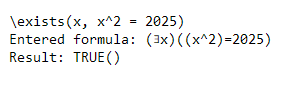
\includegraphics[width=0.99\linewidth]{пример1.PNG} \\ а)}
    \end{minipage}
    \hfill
    \begin{minipage}[ht]{0.4\linewidth}
        \center{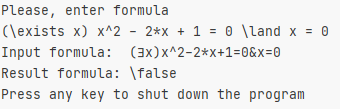
\includegraphics[width=0.99\linewidth]{пример2.PNG} \\ б)}
    \end{minipage}
    \\
    \begin{minipage}[ht]{0.4\linewidth}
        \center{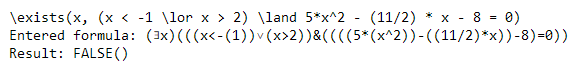
\includegraphics[width=0.99\linewidth]{пример3.PNG} \\ в)}
    \end{minipage}
    \hfill
    \begin{minipage}[ht]{0.4\linewidth}
        \center{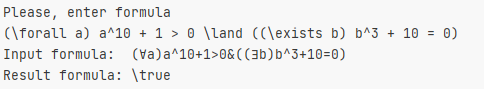
\includegraphics[width=0.99\linewidth]{пример4.PNG} \\ г)}
    \end{minipage} 
    \label{fig:примеры}
\end{figure}

\subsection{О возможных приложениях}
Несколько слов скажем о возможных приложениях написанной нами программы.

Во-первых, благодаря гибкой архитектуре, слабым связям между модулями через интерфейсы, данный программный комплекс можно расширять, добавлять в него новые правила грамматики, новый преобразователи формул, тем самым расширяя язык и способы эквивалентных преобразований.

Во-вторых, идет активное развитие систем автоматической верификации программ и моделей безопасности. Если сформулировать требования к их безопасности на формальном языке, то примерно теми же методами можно доказывать их соответствие заявленным требованиям и безопасность. 
